\section{Numerische Lösung nichtlinearer Gleichungssysteme}

\begin{remark}
    In diesem Kapitel geht es um die Nullstellenbestimmung von\\ nichtlinearen Funktionen $f: \R^n \to \R^n$. \\
    Abkürzung: NLGS = nichtlineares Gleichungssystem
\end{remark}

\begin{example2}{Einleitendes Beispiel}
    $$f_1(x_1, x_2) = x_1^2 + x_2 - 11 = 0$$
    $$f_2(x_1, x_2) = x_1 + x_2^2 - 7 = 0$$
    Gesucht sind die Lösungen des Gleichungssystems. Diese lassen sich interpretieren als die Nullstellen der Funktion $\textbf{f}: \R^2 \to \R^2$ gemäss:
    $$\textbf{f}(x) = \begin{pmatrix} f_1 (x_1, x_2) \\ f_2 (x_1, x_2) \end{pmatrix} = \begin{pmatrix} x_1^2 + x_2 - 11 \\ x_1 + x_2^2 - 7 \end{pmatrix} = \begin{pmatrix} 0\\ 0 \end{pmatrix}$$
    Offensichtlich lässt sich ein solches System nicht in die Form $Ax = b$ bringen. 

    \begin{minipage}{0.5\linewidth}
    Geometrisch lassen sich die Lösungen als Schnittpunkte der beiden Funktionen interpretieren.\\
    Explizite Darstellung der Kurven:
    $$x_2 = 11 - x_1^2$$
    $$x_2 = \sqrt{7 - x_1}$$
    Schnittpunkte:
    $$\overline{\textbf{x}_1} = \begin{psmallmatrix} 3 \\ 2 \end{psmallmatrix}, \quad \overline{\textbf{x}_2} = \begin{psmallmatrix} -2.8 \\ 3.2 \end{psmallmatrix}$$
    $$\overline{\textbf{x}_3} = \begin{psmallmatrix} -3.8 \\ -3.3 \end{psmallmatrix}, \quad \overline{\textbf{x}_4} = \begin{psmallmatrix} 3.4 \\ -1.7 \end{psmallmatrix}$$
    \end{minipage}
    \begin{minipage}{0.5\linewidth}
    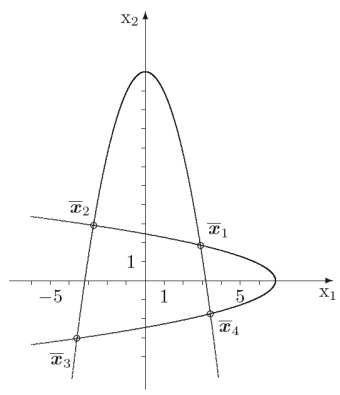
\includegraphics[width=\linewidth]{einleitendes_bsp_kap5.png}
    \end{minipage}
\end{example2}

\subsection{Funktionen mit mehreren Variablen}

\begin{lemma}{Funktion} mit abhängiger Variable $x$, unabhängiger Variable $y$ = $f(x)$:
    $$f: \R \to \R$$
    $$\quad x \mapsto f(x)$$
\end{lemma}

\begin{definition}{Skalarwertige Funktionen mit mehreren Variablen}
    $$f: D \subset \R^n \to W \subset \R$$
    $$(x_1, x_2, \ldots, x_n) \mapsto y = f(x_1, x_2, \ldots, x_n)$$
    Unter einer Funktion $f$ mit $n$ unabhängigen Variablen $x_1, \ldots, x_n$ und einer abhängigen Variablen $y$ versteht man eine Vorschrift, 
    die jedem geordneten Zahlentupel $(x_1, x_2, \ldots, x_n)$ aus einer Definitionsmenge $D \subset \R^n$ genau ein Element $y \in W \subset \R$ zuordnet.
    \vspace{2mm} \\
    Da das Ergebnis $y \in \R$ ein Skalar (eine Zahl) ist, redet man auch von einer \textbf{skalarwertigen Funktion}.
\end{definition}

\begin{concept}{Vektorwertige Funktion} Erweiterung der obigen Definition, gibt einen \textbf{Vektor} zurück (anstatt eines Skalars).\\
    Sei $\textbf{f}: \R^n \to \R^m$ eine Funktion mit $n$ Variablen. Dann ist die Funktion $\textbf{f}$ definiert durch:
    $$\textbf{f}(x_1 \ldots, x_n) = \begin{pmatrix} y_1 = f_1(x_1, x_2, \ldots, x_n) \\ y_2 = f_2(x_1, x_2, \ldots, x_n) \\ \vdots \\ y_m = f_m(x_1, x_2, \ldots, x_n) \end{pmatrix}$$
    wobei die $m$ Komponenten $f_i: \R^n \to \R$ für $i = 1, 2, \ldots, n$ von $\textbf{f}$ wieder \textbf{skalarwertige} Funktionen sind.
\end{concept}

\begin{corollary}{Eigenschaften von skalar- und vektorwertigen Funktionen}
    \begin{itemize}
        \item Skalar- und vektorwertige Funktionen mit mehreren Variablen werden auch \textbf{multivariat} genannt.
        \item Wie bei einem Vektor $\textbf{x}$ stellen wir zur besseren Unterscheidbarkeit vektorwertige Funktionen $\textbf{f}$ fett dar, im Gegensatz zu Skalaren $x$ und skalarwertigen Funktionen $f$.
        \item Wir werden uns bei der Lösung nichtlinearer Gleichungssysteme auf vektorwertige Funktionen $\textbf{f} = \R^n \to \R^n$ konzentrieren.
    \end{itemize}
\end{corollary}

\paragraph{Beispiele}

\begin{example2}{Grundlegende Rechenoperationen} können als Skalarwertige Funktionen $f: \R^2 \to \R$ oder als Vektorwertige Funktionen $\textbf{f}: \R^2 \to \R^2$ interpretiert werden
    $$f(x, y) = x + y, \quad g(x, y) = x \cdot y, \quad h(x, y) = x^2 + y^2$$
    $$\textbf{f}(x, y) = \begin{pmatrix} x + y \\ x \cdot y \end{pmatrix}, \quad \textbf{g}(x, y) = \begin{pmatrix} x \cdot y \\ x^2 + y^2 \end{pmatrix}$$
\end{example2}

\begin{example2}{Zusammenhang mit der Elektrotechnik}
    \paragraph{Ohmsches Gesetz}
    Die an einem ohmschen Widerstand $R$ abfallende Spannung $U$ hängt vom Widerstand $R$ und der Stromstärke $I$ gemäss dem ohmschen Gesetz $U=R \cdot I$ ab. Also haben wir für die abhängige Variable $U=f(R, I)=R I$ die skalarwertige Funktion $f: \mathbb{R}^2 \longrightarrow \mathbb{R}$ mit den unabhängigen Variablen $R$ und $I$. Häufig schreibt man auch direkt
    $$
    U=U(R, I)=R \cdot I
    $$
    und bringt dadurch die Abhängigkeit der Variable $U$ von den unabhängigen Variablen $R$ und $I$ zum Ausdruck, wie wir es auch bereits vom eindimensionalen Fall kennen, z.B. $y=y(x)$.

    \paragraph{Reihenschaltung von Widerständen}
    Bei der Reihenschaltung von $n$ ohmschen Widerständen $R_1, R_2, \ldots, R_n$ ergibt sich der Gesamtwiderstand $R$ gemäss
    $$
    R=R(R_1, R_2, \ldots, R_n)=R_1+R_2+\ldots+R_n
    $$    
\end{example2}

\begin{example2}{lineare Funktionen von LGS}
    Gebe die lineare Funktion $\textbf{f}: \R^3 \to \R^3$ an, für welche die Lösung $\textbf{x}$ des LGS:
    $$\textbf{Ax} = \textbf{b} \text{ mit } \textbf{A} = \begin{pmatrix} 4 & -1 & 1 \\ -2 & 5 & 1 \\ 1 & -2 & 5 \end{pmatrix} \text{ und } \textbf{b} = \begin{pmatrix} 1 \\ 2 \\ 3 \end{pmatrix}$$
    gerade $\textbf{f(x)} = \textbf{0}$ ergibt.
    \vspace{2mm} \\
    \textbf{Vorgehen}: \\
    $$\overrightarrow{\textbf{f}}(x_1, x_2, x_3) = 0 \begin{pmatrix} x_1 \\ x_2 \\ x_3 \end{pmatrix} = \begin{pmatrix} 0 \\ 0 \\ 0 \end{pmatrix}$$
    $$\textbf{A} \overrightarrow{\textbf{x}} = \overrightarrow{\textbf{b}} \Rightarrow \underbrace{\textbf{A} \overrightarrow{\textbf{x}} - \overrightarrow{\textbf{b}} = \overrightarrow{\textbf{0}}}_{\overrightarrow{\textbf{f}}(\overrightarrow{\textbf{x}})}$$
    \tcblower
    $$\overrightarrow{\textbf{f}}(\overrightarrow{\textbf{x}}) = \textbf{A} \overrightarrow{\textbf{x}} - \overrightarrow{\textbf{b}} = \begin{pmatrix} 4 & -1 & 1 \\ -2 & 5 & 1 \\ 1 & -2 & 5 \end{pmatrix} \begin{pmatrix} x_1 \\ x_2 \\ x_3 \end{pmatrix} - \begin{pmatrix} 5 \\ 11 \\ 12 \end{pmatrix}$$
    Die Funktion $\textbf{f}$ ist gegeben durch: (\textcolor{pink}{\textbf{solved by copilot so no guarantees}})
    $$\textbf{f}(x_1, x_2, x_3) = \begin{pmatrix} f_1 = 4x_1 - x_2 + x_3 - 5 \\ f_2 = -2x_1 + 5x_2 + x_3 - 11 \\ f_3 = x_1 - 2x_2 + 5x_3 - 12 \end{pmatrix}$$
\end{example2}

\subsubsection{Darstellungsformen}

\begin{concept}{Analytische Darstellung}
    \begin{itemize}
        \item \textbf{Explizite Darstellung:} $y = f(x_1, \ldots, x_n)$
        \begin{itemize}
            \item die Funktionsgleichung ist nach einer Variablen aufgelöst
            \item Beispiel: $y = 2 \cdot e^(x_1^2 + x_2^2)$
        \end{itemize}
        \item \textbf{Implizite Darstellung:} $F(x, y) = 0$
        \begin{itemize}
            \item die Funktionsgleichung ist nicht nach einer Variablen aufgelöst
            \item daher handelt es sich um eine Funktion mit nur $n-1$ unabhängigen Variablen
            \item Beispiel: $x_1^2 + x_2^2 - 1 = 0$
        \end{itemize}
        \item \textbf{Parameterdarstellung:} $x = x(t), y = y(t)$
        \begin{itemize}
            \item die Funktion wird durch eine Kurve im Raum beschrieben
            \item Beispiel: $x(t) = \cos(t), y(t) = \sin(t)$
        \end{itemize}
    \end{itemize}
\end{concept}

\begin{concept}{Darstellung durch Wertetabelle}
    Sei $f: \R^n \to \R^m$ eine Funktion.\\
    \textbf{Vorgehen:}\\
    In die vorausgesetzte Funktionsgleichung $z = f(x,y)$ werden die Werte der unabhängigen Variablen $x$ und $y$ eingesetzt (der Reihe nach).\\
    So erhält man eine Wertetabelle, bzw. Matrix:\\
    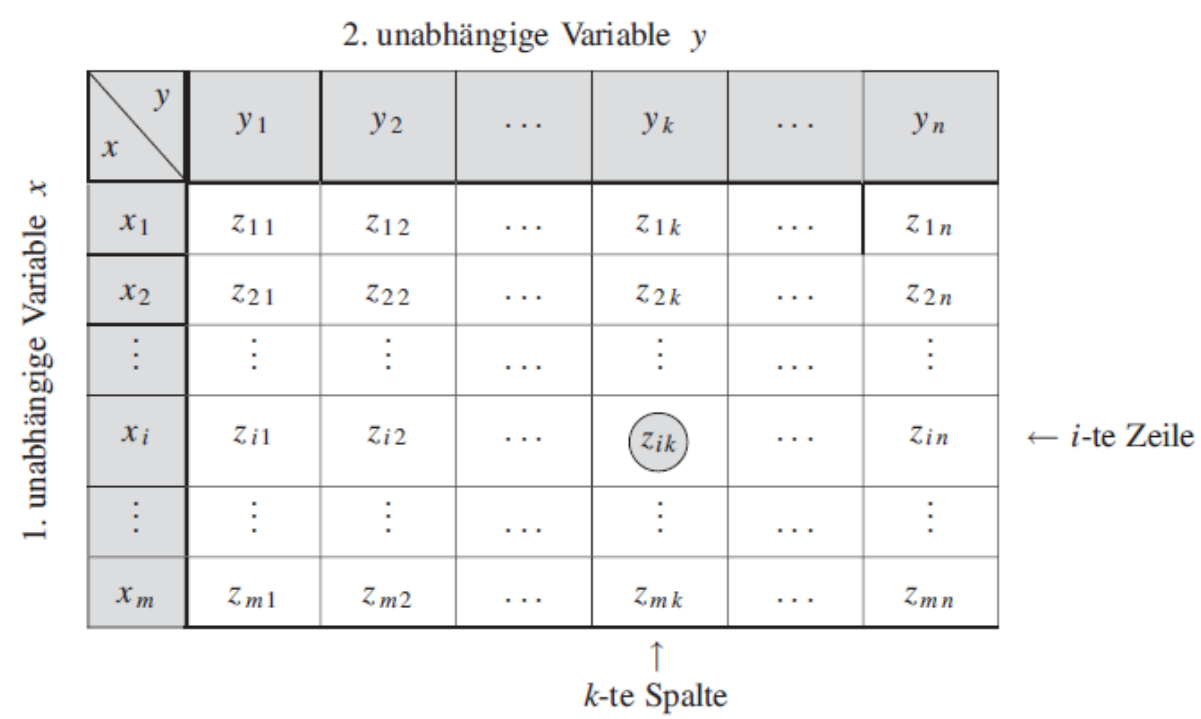
\includegraphics[width=\linewidth]{wertetabelle_darstellung.png}
\end{concept}

\begin{concept}{Grafische Darstellung}
    Wir beschränken uns hier auf skalarwertige Funktionen mit zwei unabhängigen Variablen $f: \R^2 \to \R$.\\
    Dazu betrachten wir die Funktion $z = f(x, y)$ in einem dreidimensionalen kartesischen Koordinatensystem:
    
    \paragraph{Darstellung einer Funktion als Fläche im Raum}
    Die Funktion $f$ ordnet jedem Punkt $(x, y) \in D$ in der Ebene einen Wert $z=f(x, y)$ zu, der als Höhenkoordinate verstanden werden kann. 
    Durch die Anordnung der Punkte ( $x, y, f(x, y)$ ) im dreidimensionalen Koordinatensystem wird eine über dem Definitionsbereich $D$ liegende Fläche ausgezeichnet:

    \includegraphics[width=\linewidth]{funktion_als_fläche_im_raum.png}
    
    \paragraph{Schnittkurvendiagramm}
    Wird die Fläche $z=f(x, y)$ bei einer konstanten Höhe $z=$ const. geschnitten, ergibt sich eine Schnittkurve. 
    Wird diese in die $(x, y)$-Ebene projiziert, spricht man von einer Höhenlinie bzw. bei der Abbildung von einem Höhenliniendiagramm., wie wir es z.B. von Wanderkarten her kennen. 
    Natürlich kann man auch andere Schnitte als $z=$ const. (Schnittebene parallel zur $(x, y)$-Ebene) wählen, z.B. $x=$ const. (Schnittebene parallel zur $(y, z)$-Ebene) oder $y=$ const. (Schnittebene parallel zur $(x, z)$-Ebene):

    \begin{minipage}{0.6\linewidth}
    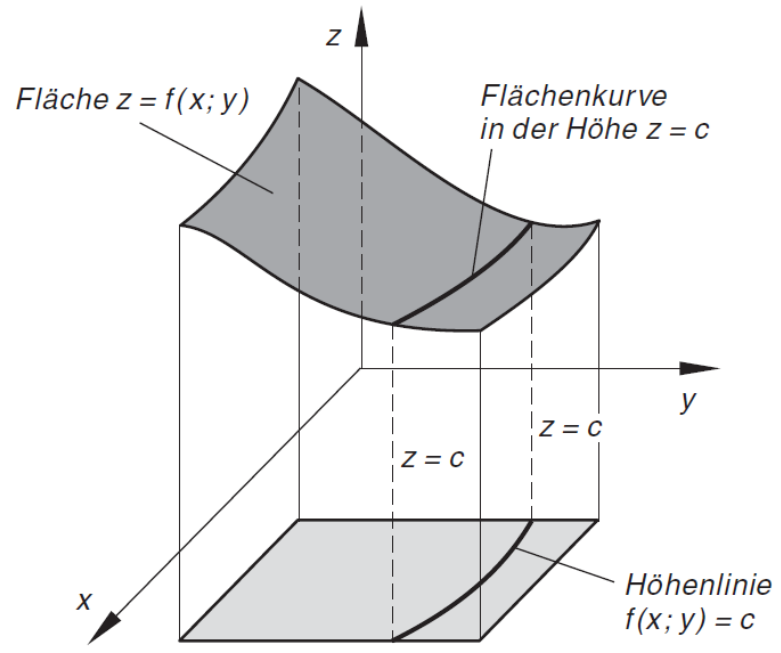
\includegraphics[width=\linewidth]{grafische_darstellung_detailed.png}
    \end{minipage}
    \begin{minipage}{0.38\linewidth}
    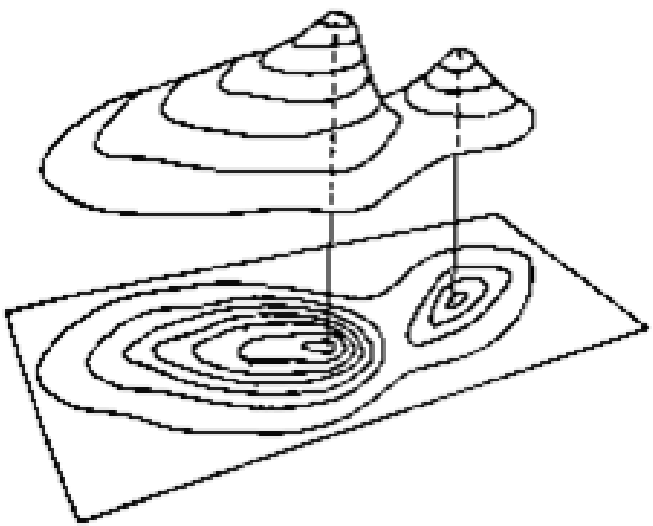
\includegraphics[width=\linewidth]{grafische_darstellung2.png}\\
    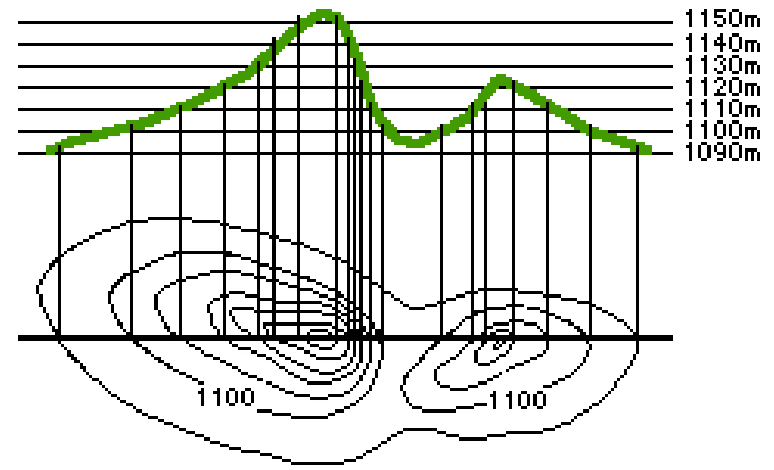
\includegraphics[width=\linewidth]{grafische_darstellung3.png}
    \end{minipage}
\end{concept}

